\documentclass[11pt]{article}

\usepackage{calc}
\usepackage{graphicx}
\graphicspath{ {images/} }

\usepackage{relsize}
\usepackage{multirow}
\usepackage{bm}
\usepackage{enumitem}
\usepackage{multicol}
\usepackage{parcolumns}
\usepackage{array}
\usepackage{hhline}
\usepackage{url}
\usepackage{titling}
\usepackage{forest}

\usepackage{hyperref}
\hypersetup{
    colorlinks = true,
    linkcolor = {red},
    citecolor = {blue}
}

\usepackage{breakurl}
\usepackage{geometry}

%%%%%%%%%%%%%%%%
%Font packages

\usepackage[T1]{fontenc}

%Times New Roman
%\usepackage{mathptmx}

%Euler math fornts
%\usepackage[small]{eulervm}

%Charter
\usepackage{charter}

%Palatino
%\usepackage{palatino}


%IPA package
\usepackage{tipa}



%International
\usepackage{CJKutf8}
\usepackage[german, russian, USenglish]{babel}

\usepackage[normalem]{ulem}

%CJK Environments
\newenvironment{SChinese}{%
  \CJKfamily{gbsn}%
  \CJKtilde
  \CJKnospace}{}
\newenvironment{TChinese}{%
  \CJKfamily{bsmi}%
  \CJKtilde
  \CJKnospace}{}
\newenvironment{Japanese}{%
  \CJKfamily{min}%
  \CJKtilde
  \CJKnospace}{}
\newenvironment{Korean}{%
  \CJKfamily{mj}}{}


%Funny symbols
\usepackage{pifont}
\newcommand{\checkmark}{\ding{51}}
\newcommand{\crossmark}{\ding{55}}

%Examples packages
\usepackage{linguex}
\usepackage{cgloss}
			

%Standard stuff
\usepackage{amsmath,amssymb}
\usepackage[sort]{natbib}
\usepackage{natbibspacing}
\usepackage{multirow,enumerate}

%Hyperlinks

% PST-JTREE packages
\usepackage{pstricks}
\usepackage{pst-xkey}
\usepackage{pst-jtree}


\geometry{letterpaper,includehead,includefoot,margin=2cm}

\def\labelBr#1 {\mbox{$\hspace{.05em}\ind{\mbox{\scriptsize\sc#1}}$} }

\renewcommand{\baselinestretch}{1.0}


\bibpunct{(}{)}{;}{a}{,}{,}

\newcommand{\citeposs}[1]{\citeauthor{#1}'s \citeyear{#1}}

\newcommand{\twoline}[2]{\begin{tabular}{c}{#1}\\{#2}\end{tabular}}

\newcommand{\dict}[2]{\emph{#1} `#2'}

\newcommand{\morph}[1]{\textsc{#1}}

\newcommand{\indgl}[1]{$\sb\text{\textsc{#1}}$}

\newcommand{\ind}[1]{\ifmmode\sb{#1}\else$\sb{\text{#1}}$\fi}


\newcommand{\angb}[1]{$\left<\text{#1}\right>$}

\newcommand{\trc}{\underline{\phantom{aaa}}}
\newcommand{\ttt}{\texttt{t}}


\newcommand{\1}{$'$}
\newcommand{\2}{$''$}
\newcommand{\3}{$'''$}

%\pagestyle{fancy}

\newcommand{\compresslist}{%
\setlength{\itemsep}{1pt}%
\setlength{\parskip}{0pt}%
\setlength{\parsep}{0pt}%
}

\newcommand{\exhead}{\\*\clubpenalty=10000}
\newcommand{\headpenalty}{\clubpenalty=10000}

%%%% Paragraph with a new line %%%%
\makeatletter
\renewcommand\paragraph{%
\@startsection {paragraph}
{4}
{0pt}
%{3.25ex plus 1ex minus .2ex} % indentation
{-3.25ex plus 1ex minus .2ex} % no indentation
%{-1em} % no new line
{1em} % new line
{\normalfont \normalsize \bfseries }%
}
\makeatother


%%%% Subsubsubsections %%%%
\setcounter{secnumdepth}{5}
\setcounter{tocdepth}{5}
%\titlespacing*{\paragraph}    {0pt}{3.25ex plus 1ex minus .2ex}{1.5ex plus .2ex}

%------


%\author{}%
\title{New York City English}%


\begin{document}

%\maketitle %

%\renewcommand{\baselinestretch}{1.5}

\begin{center}
\LARGE\textbf{\thetitle}
\end{center}


\tableofcontents

\section{Introduction}

New York City English is a well studied dialect, the first publication is \citealp{Babbitt:1896}. First major linguistic study is \citealp{Labov:1966} and its second edition \citealp{Labov:2006}.

\section{\citeauthor{Labov:1966}'s study}

Description of the main features of New York English:

\subsection{\emph{R}-lessness}

	 \textbf{r-variable:} \textipa{[\*r]} is deleted/pronounced like a vowel in syllable coda\footnote{\textbf{Syllable coda} is a part of the syllable that comes after a vowel. For example, in the monosyllabic word \emph{plant} the coda is \emph{nt}. The part of the syllable that comes before the vowel is called an \textbf{onset}: in \emph{plant}, the onset is \emph{pl}.
		
		\begin{center}
			\begin{forest}
				[Syllable, for tree={parent anchor=south, child anchor=north}
					[Onset[pl,tier=word]]
					[Rhyme
						[Nucleus[a,tier=word]]
						[Coda[nt,tier=word]]	
					]
				]	
			\end{forest}
	
		\end{center}

	} position. This feature is often referred to as \emph{r-lessness}, and dialects which use this features are called \emph{r-less}, or \emph{non-rhotic}.
	

\begin{tabular}{ l c c }
\hline
Spelling & Mainstream Pronunciation & New York Pronunciation\\ \hline
car & \textipa{[kA\*r]} & \textipa{[kA:]}\\
careful & \textipa{[kE\*rfUl]} & \textipa{[kE:fUl]}\\ \hline
\end{tabular}

\vspace{1em}

\textbf{Origin:} British English, brought to the US by British settlers to the entire Eastern Seaboard.

\textbf{\citealp{Labov:1966}'s findings:} Factors influencing \emph{r-lessness}:

\begin{itemize}
\item Class and socioeconomic status determines the frequency of r-less pronunciations: more prominent among lower class.

\begin{center}
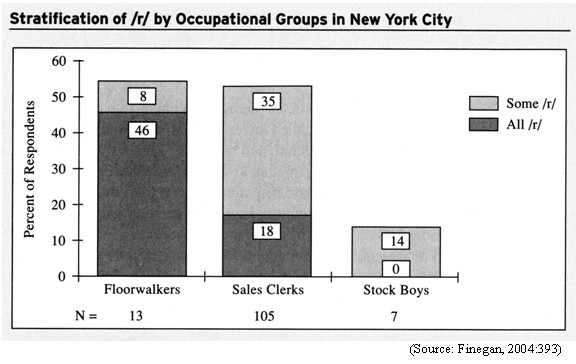
\includegraphics[width=.7\textwidth]{stratification}
\end{center}

\item Gender: males are more r-less.

\begin{center}
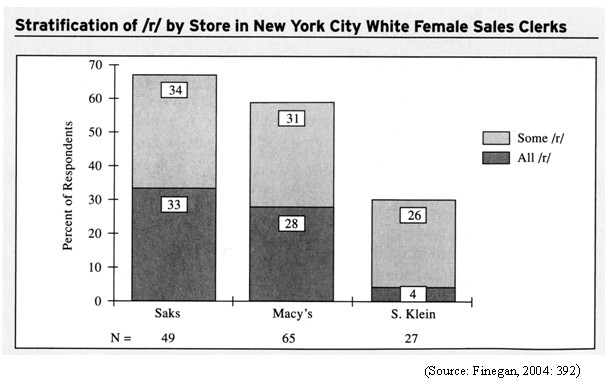
\includegraphics[width=.7\textwidth]{classpatternlabov2}
\end{center}
\end{itemize}

\noindent \textbf{Change:} r-less pronunciation is going away. Currently this is still a change in progress; more and more speakers produce \emph{r}'s, but some stick to the classical pronunciation.

\subsection{\emph{Coffee/Thought}-vowel}

\textbf{\emph{coffee}-vowel:} Low back rounded vowel \textipa{[0]} in NY City English is raising and merging with \textipa{[o]}, while in the most of the other places in the USA it is lowering towards \textipa{[6]}.

\begin{center}
	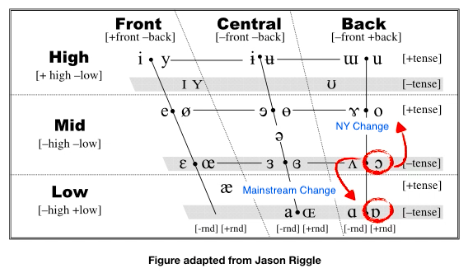
\includegraphics[width=.7\textwidth]{coffee.png}	
\end{center}

	\noindent It occurs in words like \emph{coffee}, \emph{thought}.
	
\noindent \textbf{Change:} During Labov's study, it was becoming more and more prominent feature (unlike \emph{r}-lessness!). Currently, according to Becker, this feature is decreasing in popularity.

\subsection{Short \emph{a}-split}

\textbf{Short \emph{a}-split:} in some contexts, the vowel \emph{a} stays as in Mainstream US English, and in some cases it tenses, fronts, and raises. 

	\begin{itemize}
		\item Before front nasal(\emph{n}, \emph{m}): \emph{ban}, \emph{ram}, but not \emph{bang}, \emph{rang}.
		\item Before voiceless fricatives (\emph{f}, \emph{\textipa{T}}, \emph{s}, \emph{\textipa{S}}, etc.): \emph{bath}, \emph{pass}
		\item Before voiced stops (\emph{b}, \emph{d}, \emph{g}): \emph{mad}, \emph{bag}, but not \emph{back}, \emph{Matt}.
	\end{itemize}
	
	Rules do not operate if:
	\begin{itemize}
		\item Vowel is word-initial: \emph{Ann}
		\item Open syllable\footnote{\textbf{Open syllable} are syllables with no codas, i.e. syllable that end in a vowel.}: \emph{man}, but not \emph{manner}
	\end{itemize}

\noindent \textbf{Change:} We are seeing a move away from this classic system. Younger New Yorkers only apply this rule before nasals (\emph{hang},\emph{man}), but not in other contexts.

\section{Future of the NY City English}

\subsection{Stigmatization}

NY City English is one of the most \emph{stigmatized} dialects of American English: it often gets low rankings on reception of \emph{correctness} or \emph{pleasantness} (\citealp{FridlandBartless:2006}):

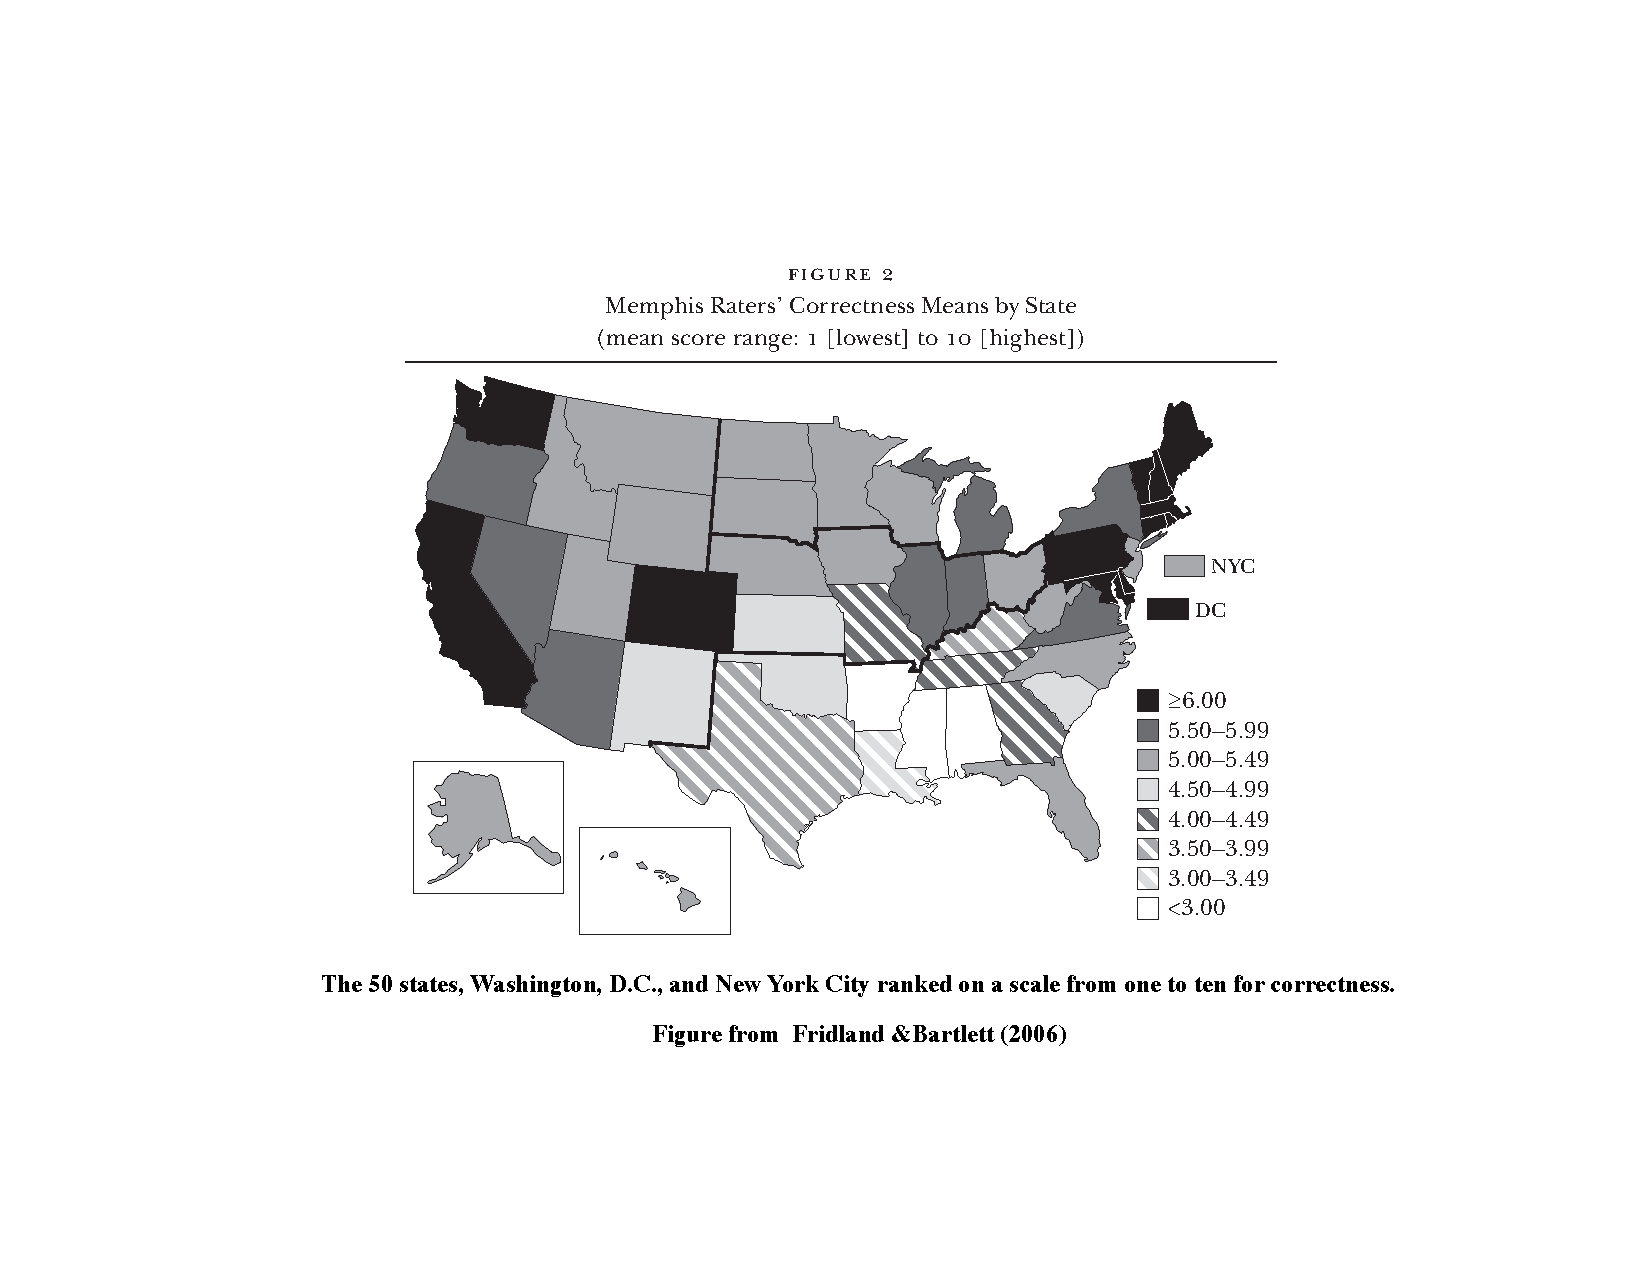
\includegraphics[width=.45\textwidth]{ratings1}\vrule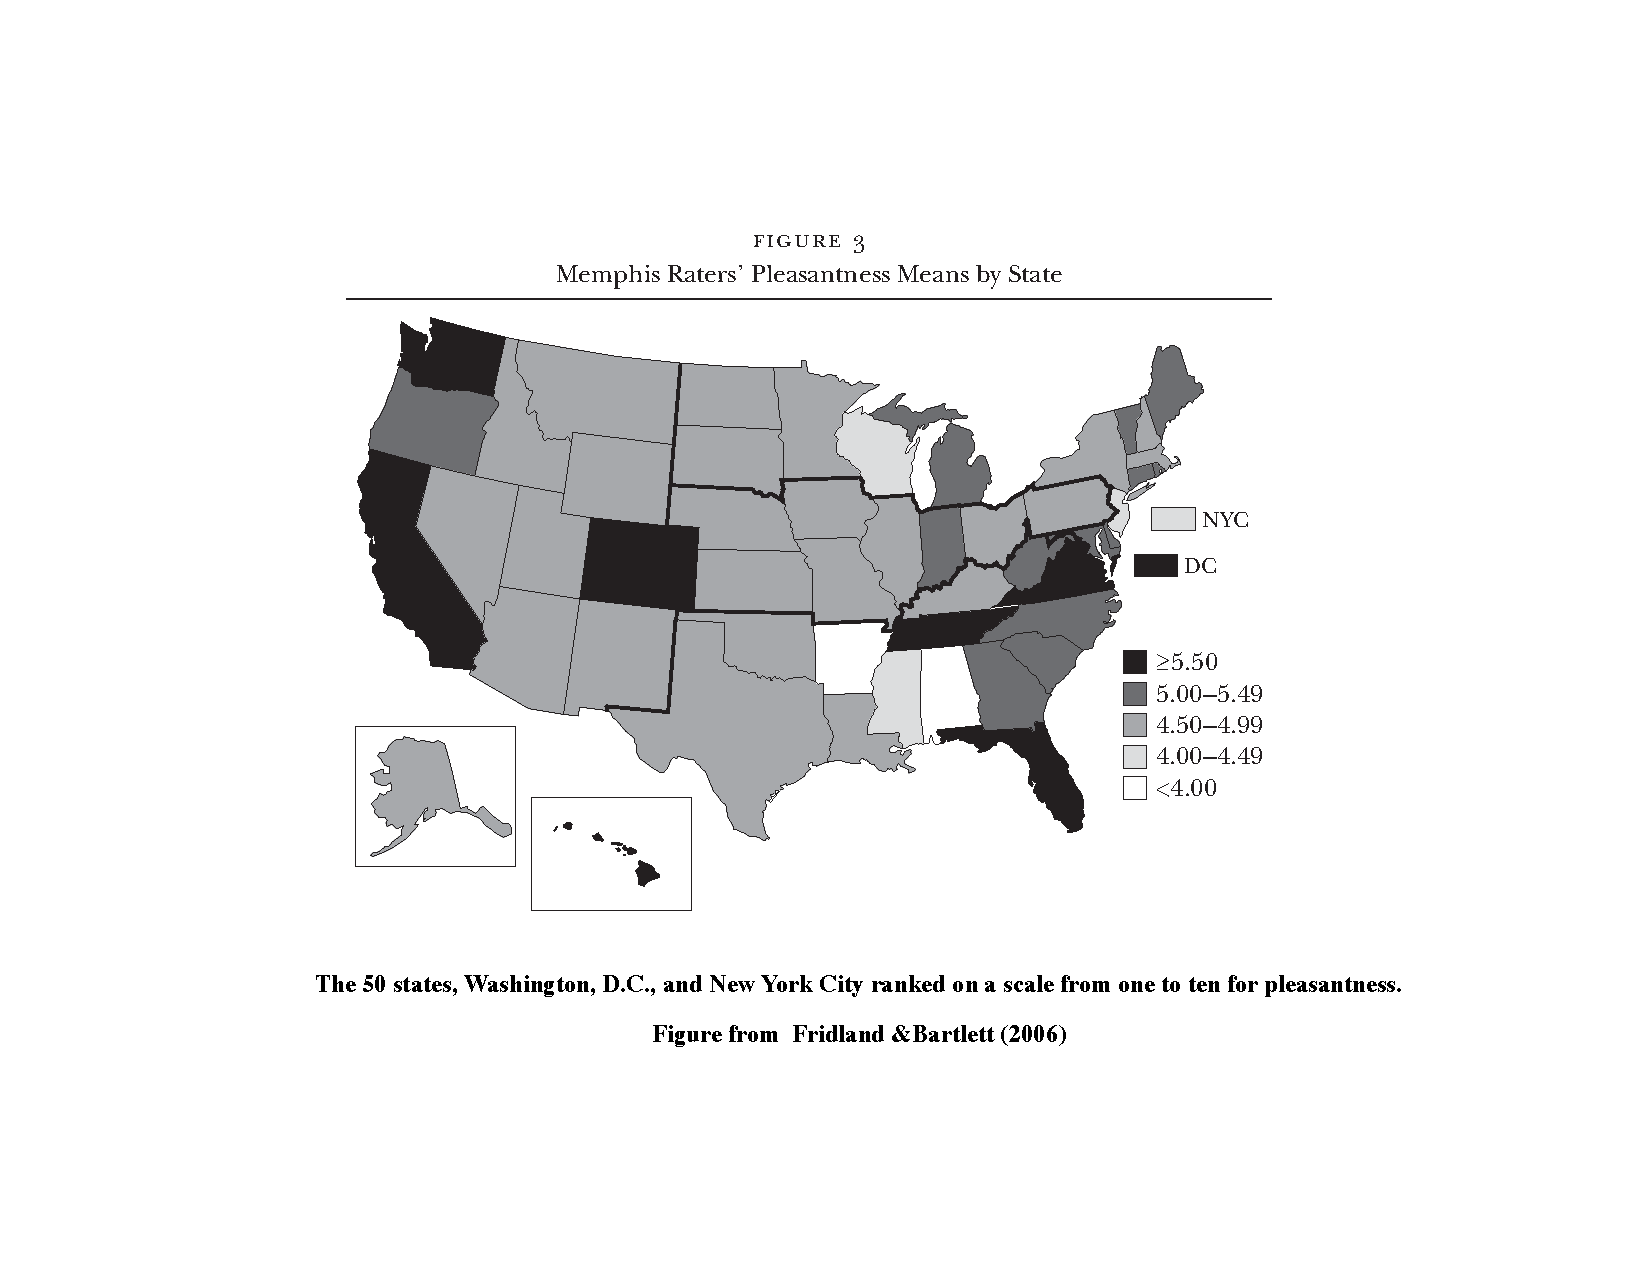
\includegraphics[width=.45\textwidth]{ratings2}

\noindent New Yorkers are aware of this stigmatization, and react to it: speakers consciously or subconsciously switch away from classic New York features.

\subsection{Recession}

Classic features are in recession, but the dialect is not disappearing, contrary to some \#BadLinguistics media publications (i.e. \citealp{Fuhgeddaboudit:2015}).

\subsection{Group Differences}

Some subgroups of the NY population are maintaining some classic features, while others are moving away from them.

\begin{itemize}
\item African-Americans are maintaining the \emph{coffee}-vowel.	
\end{itemize}

\subsection{Change?}

While three classic features are in recession, it is possible that new features will appear in NY City English and be used by the New-Yorkers to project their identity.

\section{Questions}

\begin{itemize}
\item Can you think of how NY City speech changes? 
\item Do you see any innovations and changes in NY City English? 
\item If you are from NY area, do you speak differently than your parents or grandparents?
\item Which popular movies and movie characters speak NY City dialect? Is their character in any way correlated with their accent?
\item Are there any other NY City English features that you are aware of?
\item Do you notice any other group differences than the ones already mentioned in the video? Think about social class, ethnicity, gender, age, geographic location.
\end{itemize}


\bibliographystyle{linquiry2}




\bibliography{../Bibliography/LIN200}

\end{document}
